\documentclass[12pt]{article}

\usepackage{booktabs}
\usepackage{natbib}
\usepackage{graphicx}
\usepackage{subcaption}
\usepackage{amsmath}
\usepackage{setspace}
\usepackage[margin=1in]{geometry}
\usepackage[hidelinks]{hyperref}

\widowpenalty10000
\clubpenalty10000

\graphicspath{{../../output/}}

\title{Do People Ask AI About Upcoming Elections?\\
\large Evidence from Staggered 2026 Primaries in AI Assistant and Search Data}
\author{Daniel M. Thompson\thanks{Department of Political Science, UCLA. Draft prepared July 2026. Claude usage data are from the public Anthropic Economic Index; search data are from Google Trends.}}
\date{\today}

\begin{document}

\maketitle

\begin{abstract}
\noindent Millions of Americans now use AI assistants to find information, raising the question of whether these tools are becoming part of how citizens learn about elections. I study whether people turn to an AI assistant when their state holds an election, comparing the response to the standard benchmark for information demand, Google search. I combine newly released public data on the topic composition of Claude conversations by state and month with weekly state-level Google search interest, using the staggered timing of the 2026 statewide primaries as a source of variation in when election information becomes relevant. Both series respond. Google searches for ``primary election'' rise roughly fifteen-fold between two months out and the week of a state's primary, then revert within two weeks. In the same months, the share of a state's Claude conversations about politics rises by 0.10 percentage points (s.e.\ 0.04) when the state holds its primary---a 22 percent increase over the 0.48 percent base rate in later-primary states. These results suggest AI assistants are already a measurable, though still second-order, channel through which citizens research upcoming elections.
\end{abstract}

\onehalfspacing

\section*{Introduction}

Search engines have long been the first stop for citizens looking up when to vote, what is on the ballot, and who is running. A growing share of that information seeking may now be moving to AI assistants: industry surveys report that chatbots are among the fastest-adopted consumer technologies in history, and AI developers have built dedicated election-information safeguards in anticipation of exactly this use.\footnote{Anthropic, OpenAI, and Google all announced election-specific policies for their assistants ahead of the 2024 and 2026 cycles.} Skeptics counter that assistant usage is dominated by work tasks---writing, coding, and analysis---and that for time-sensitive civic facts people still default to search \citep{handa2025economic}. Do citizens actually turn to AI assistants when their own election arrives?

Answering this question is hard because AI usage data are proprietary and individual conversations are private. I overcome this constraint with the Anthropic Economic Index (AEI), a public release of anonymized, aggregated Claude usage that reports the topic composition of conversations by U.S. state, most recently at a monthly frequency (April and May 2026). I combine these data with the natural experiment embedded in the American electoral calendar: the 2026 statewide primaries were spread across March through September, so different states' residents needed election information in different months. Eight states in the balanced AEI panel held primaries in May 2026; twenty-two comparison states voted later in the summer. I estimate a difference-in-differences comparing the politics-topic share of conversations in April versus May across the two groups, and I benchmark the result against an event study of weekly Google search interest in ``primary election'' across all fifty states and the District of Columbia over the 56 weeks from July 2025 through July 2026.

Both information channels respond to the primary calendar. Google search interest in ``primary election'' builds gradually over the six weeks before a state's primary as early voting begins, spikes in the primary week at roughly 15 times its level two months earlier, and returns to baseline within two weeks. Claude conversations shift the same way: when a state holds its May primary, the share of its conversations about politics and public records rises by 0.10 percentage points (clustered s.e.\ 0.04) relative to later-primary states, a 22 percent increase over those states' 0.48 percent May average. The estimate is similar when I drop June-primary states, whose mail-ballot period begins in May, from the comparison group (0.09 points), and in logs (a 27 percent increase, s.e.\ 9 percent).

Two additional patterns support the interpretation that this is election-driven information seeking rather than chance topical drift. First, the AEI's finest-grained ``Elections'' conversation topic clears the dataset's privacy-based publication threshold in only three states in April 2026 but eight in May---and the states it newly appears in are disproportionately May-primary states like Oregon, Pennsylvania, and Georgia. Second, in the national time series, the election-related conversation share is highest in the observation window immediately following the November 2025 elections and rises again between April and May 2026 as the primary season builds.

This note contributes to two literatures. A rapidly growing body of work uses aggregated assistant-usage data to describe what people do with AI \citep{handa2025economic, tomlinson2025working}, but has focused on work tasks and adoption gaps rather than civic information. A separate literature uses search data to measure the public's demand for election information \citep{stephensdavidowitz2014cost, trevisan2018search}. I connect the two, providing what is to my knowledge the first causally identified estimate of how AI assistant usage responds to an election.

The design has clear limits. The AEI state-by-month panel covers only two months, so the identifying comparison is a single pre/post contrast across primary cohorts; conversation topics are re-clustered in each data release, restricting analysis to within-release comparisons; and cells below a privacy threshold are unpublished, which limits the sample to 30 larger states and means the finest election-specific topic cannot be used as an outcome. The estimates describe the volume of election-related conversations, not their content or quality. And because Google Trends indices are normalized within state, the two channels' responses are comparable in proportional terms, not in levels: nothing here measures whether more people asked Claude than searched Google, only that both respond to the same electoral calendar.

\section*{Data}

\subsection*{Claude conversations by state and topic}

The Anthropic Economic Index publishes anonymized, aggregated measures of Claude chat usage, including the share of each U.S. state's conversations assigned to a hierarchy of request topics.\footnote{The data are released under a CC-BY license at \url{https://huggingface.co/datasets/Anthropic/EconomicIndex}. Conversation counts below a privacy threshold are not published.} The June 2026 release reports, for each calendar month (April and May 2026), the percent of a state's conversations in each topic. My main outcome is the share of conversations assigned to the ``Politics and public record'' topic, the broadest political category, which is published in both months for 33 states; excluding the three March-primary states leaves an analysis sample of 30, including the District of Columbia. Its detailed subtopic ``Elections'' is published for too few states to serve as an outcome---itself a consequence of the privacy threshold that I return to below. Earlier releases provide comparable national snapshots for one-week windows in August 2025, November 2025, and February 2026, which I use descriptively; because the topic taxonomy is re-estimated in each release, I never compare topic shares across releases.

\subsection*{Google search interest}

From Google Trends I collect weekly search interest in the term ``primary election'' for all fifty states and the District of Columbia over the 56 complete weeks from June 29, 2025 through July 25, 2026.\footnote{Trends reports integer indices normalized within each query batch; I collected states in eleven batches and the analysis uses only within-state variation (state fixed effects, log outcomes), which the batch normalization cannot affect. Appendix~A describes the collection and a validation exercise in detail.} The index measures the term's share of all searches in the state-week, scaled so each batch's maximum is 100.

\subsection*{The 2026 primary calendar}

I hand-compiled each state's 2026 statewide primary date from the National Conference of State Legislatures and the Federal Voting Assistance Program, which agree on every state. Primaries run from March 3 (Texas, North Carolina, Arkansas) through mid-September; eleven states voted in May, twenty in June or later. Louisiana's May 16 primary covers its U.S. Senate seat and local offices only, and Wisconsin held a separate nonpartisan spring election on April 7; results are unchanged if either state is dropped.

\section*{Design}

For the search data I estimate an event study,
\begin{equation}
\log(1 + y_{sw}) = \sum_{k \neq -1} \beta_k \mathbf{1}\{w - P_s = k\} + \alpha_s + \gamma_w + \varepsilon_{sw},
\end{equation}
where $y_{sw}$ is search interest in state $s$ and week $w$, $P_s$ is the week of state $s$'s primary, and $\alpha_s$ and $\gamma_w$ are state and week fixed effects. Event time is binned at $-9$ and $+5$ weeks, standard errors are clustered by state, and states with primaries after the sample window (August and September) contribute as not-yet-treated controls. Because treatment timing is staggered, I also report Sun-Abraham interaction-weighted estimates, which are nearly identical.

For the Claude data, with two months and two primary cohorts, the design collapses to a difference-in-differences:
\begin{equation}
y_{sm} = \delta \left(\text{May primary}_s \times \text{May}_m\right) + \alpha_s + \gamma_m + \varepsilon_{sm},
\end{equation}
where $y_{sm}$ is the politics-topic share in state $s$ and month $m \in \{\text{April}, \text{May}\}$. The identifying assumption is that absent a primary, May-primary states' conversation mix would have moved like later-primary states'. Texas, North Carolina, and Illinois held March primaries (Texas and North Carolina also held May runoffs) and are excluded as already-treated; a specification dropping June-primary control states, where mail voting begins in May, addresses anticipation.

\section*{Results}

\subsection*{Search interest spikes in the primary week}

Figure~\ref{fig:trends} shows the search response. Panel (a) plots raw mean search interest by week relative to the primary for the 31 states whose full event window falls inside the sample. Interest averages 4.5 index points seven and eight weeks out, builds steadily to 16 points in the final pre-election week as early voting begins, jumps to 68 points in the primary week---about 15 times the far-pre-period mean---and collapses to 7 points the week after. Panel (b) shows the corresponding event-study coefficients, measured relative to the week before the primary: the leads trace a steady anticipation gradient rather than a flat pre-trend, the primary week jumps by 1.10 log points (s.e.\ 0.09)---roughly a tripling relative to the already-elevated final pre-election week---and interest returns immediately to far-pre-period levels. The Sun-Abraham interaction-weighted estimates are nearly identical (primary-week effect of 1.03, s.e.\ 0.08), so staggered treatment timing is not driving the two-way fixed effects estimates.

\begin{figure}[t]
\centering
\begin{subfigure}{0.85\textwidth}

\includegraphics[width=\textwidth]{trends_raw_event_means.pdf}
\caption{Raw mean search interest by event week}
\end{subfigure}
\begin{subfigure}{0.85\textwidth}

\includegraphics[width=\textwidth]{trends_event_study.pdf}
\caption{Event-study estimates}
\end{subfigure}
\caption{\textbf{Google searches for ``primary election'' spike in the week of the state's primary.} Panel (a) shows mean search interest by week relative to the state's 2026 primary for the 31 states whose full $-8$ to $+4$ week window lies within the sample. Panel (b) shows event-study coefficients on log search interest with state and week fixed effects (circles, with 95 percent confidence intervals clustered by state) and Sun-Abraham estimates (triangles); the reference week is $-1$.}
\label{fig:trends}
\end{figure}

\subsection*{Claude conversations shift toward politics in the primary month}

Figure~\ref{fig:aei} shows the analogous pattern in AI assistant usage. Among the 22 control states with June-through-September primaries, the politics-topic share of conversations is essentially unchanged from April to May 2026 (0.48 to 0.48 percent). In the eight states that held May primaries, it rises from 0.40 to 0.50 percent. The shift is not driven by one or two states: seven of the eight May-primary states move up (panel b), with a median change of $+$0.10 percentage points, while the control states' changes straddle zero. Table~\ref{tab:aei_did} reports the corresponding estimates: 0.10 percentage points (s.e.\ 0.04), or 22 percent of the control-group mean. The estimate is 0.09 when June-primary states are dropped from the control group and implies a 27 percent proportional increase in logs.\footnote{Tennessee, a control state under this coding, holds county-office primaries in early May---visible as a May spike in its search data---so it is a conservative inclusion; dropping it gives 0.11 (s.e.\ 0.04).} With 30 states the design can detect effects of about 0.11 percentage points, so these estimates sit at the edge of detectability---the data can rule out effects twice as large, but not effects half as large.

\begin{figure}[t]
\centering
\begin{subfigure}{0.85\textwidth}
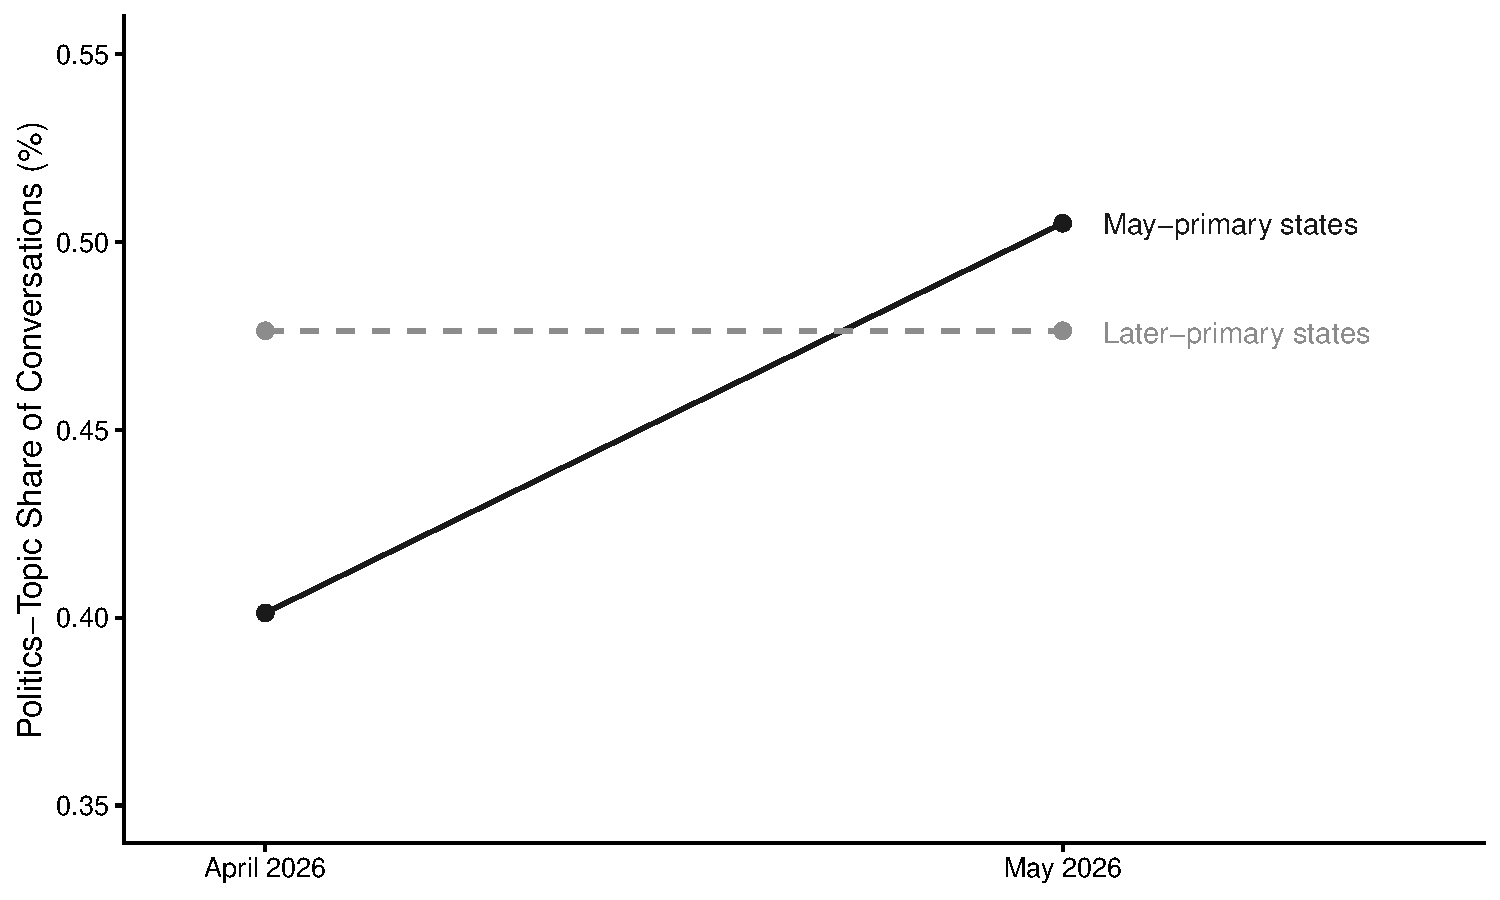
\includegraphics[width=\textwidth]{aei_politics_did.pdf}
\caption{Group means}
\end{subfigure}
\begin{subfigure}{0.85\textwidth}
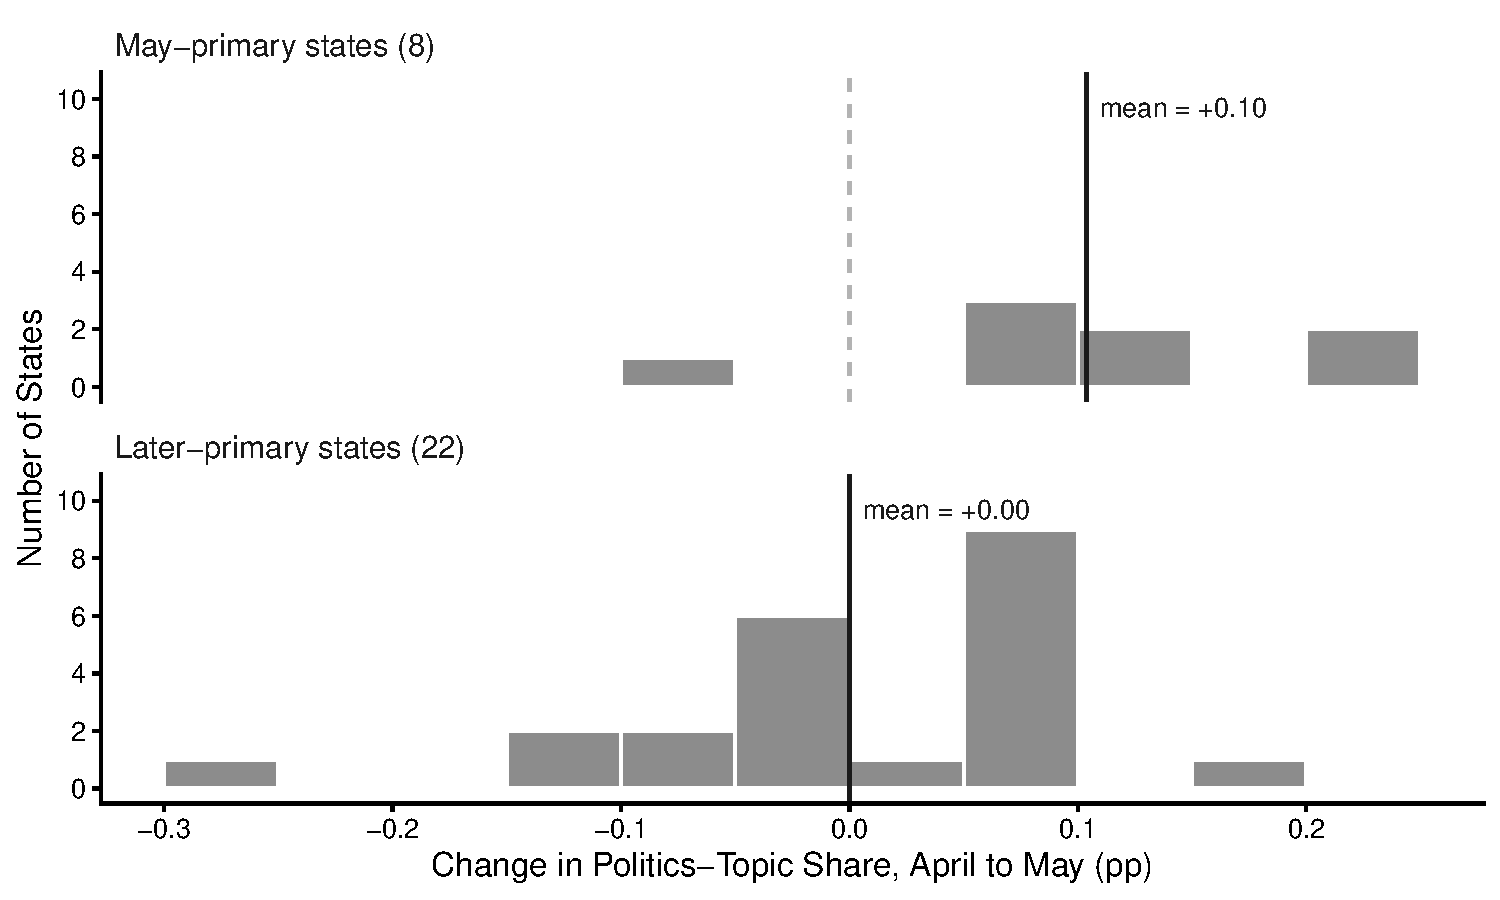
\includegraphics[width=\textwidth]{aei_change_hist.pdf}
\caption{Distribution of state-level changes}
\end{subfigure}
\caption{\textbf{The politics-topic share of Claude conversations rises when a state holds its primary.} Panel (a) plots the mean politics-topic share of conversations in April and May 2026 for the eight states with May 2026 primaries and the 22 states with June-September primaries; March-primary states are excluded. Panel (b) shows each state's April-to-May change, by group, with vertical lines at the group means.}
\label{fig:aei}
\end{figure}

\begin{table}[t]
\centering
\caption{\textbf{Claude Conversations Shift Toward Politics When a State Holds Its Primary.}\label{tab:aei_did}}
\begin{tabular}{lccc}
\toprule \toprule
 & \multicolumn{2}{c}{Politics-Topic Share (\%)} & Log Share \\
\cmidrule(lr){2-3} \cmidrule(lr){4-4}
 & (1) & (2) & (3) \\
\midrule
Primary $\times$ May & 0.10 & 0.09 & 0.24 \\
 & (0.04) & (0.04) & (0.09) \\[2mm]
\# States & 30 & 20 & 30 \\
\# Treated States & 8 & 8 & 8 \\
\# Observations & 60 & 40 & 60 \\
Control May Mean & 0.48 & 0.45 & 0.48 \\
Minimum Detectable Effect & 0.11 & 0.12 & 0.24 \\
\midrule
State Fixed Effects & Yes & Yes & Yes \\
Month Fixed Effects & Yes & Yes & Yes \\
Excl.\ June-Primary Controls & No & Yes & No \\
\bottomrule \bottomrule
\multicolumn{4}{p{0.95\textwidth}}{\footnotesize \textit{Notes}: Each column reports a difference-in-differences estimate comparing the politics-topic share of Claude conversations in April and May 2026 between states holding a statewide primary in May 2026 and states with later primaries. The outcome in columns 1 and 2 is the percent of a state's conversations assigned to the ``Politics and public record'' topic in the Anthropic Economic Index; column 3 uses its natural log. Texas, North Carolina, and Illinois, which held March primaries, are excluded. Column 2 further drops control states with June primaries, whose mail voting begins in May. Standard errors clustered by state are in parentheses. The minimum detectable effect is 2.80 times the standard error.} \\
\end{tabular}
\end{table}


Two auxiliary patterns corroborate the interpretation. First, the AEI's detailed ``Elections'' topic is published only where conversation counts clear a privacy floor; it appears in three states in April but eight in May, and the newly published states are disproportionately May-primary states (Oregon, Pennsylvania, Georgia). Election conversations became common enough to publish exactly where and when primaries occurred. Second, Figure~\ref{fig:national} places the two months in the national arc of the election cycle: the election-topic share of U.S. conversations is highest in the window just after the November 2025 elections, lower in the off-season, and rising again from April to May 2026 as the primary season builds. The same figure shows the national search series for comparison, with its unmistakable spikes at the March primaries and the peak primary weeks.

\begin{figure}[t]
\centering
\begin{subfigure}{0.85\textwidth}

\includegraphics[width=\textwidth]{national_trends_series.pdf}
\caption{Google search interest, weekly}
\end{subfigure}
\begin{subfigure}{0.85\textwidth}

\includegraphics[width=\textwidth]{national_claude_series.pdf}
\caption{Claude election-topic share, by AEI observation window}
\end{subfigure}
\caption{\textbf{Both channels track the national election calendar.} Panel (a) shows weekly U.S. search interest in ``primary election''; shaded bands mark the five AEI observation windows. Panel (b) shows the share of U.S. Claude conversations on the election-related topic in each AEI window. Topic taxonomies differ between the 2025 and 2026 releases, so points are connected only within a taxonomy; levels are not comparable across the break.}
\label{fig:national}
\end{figure}

\section*{Conclusion}

When a state's primary arrives, its residents' Claude conversations shift measurably toward politics, just as their Google searches spike---the first causally identified evidence, to my knowledge, that citizens use AI assistants to research upcoming elections. The proportional response in assistant conversations (roughly 20--25 percent) is far smaller than the many-fold spike in election-specific searches, consistent with assistants complementing rather than displacing search for time-sensitive civic facts, though the comparison is between a broad conversation-topic share and a single search term, and the normalized search index precludes level comparisons.

Beyond the substantive finding, the exercise illustrates both the promise and the current limits of public AI-usage data for social science. The AEI's state-by-month topic panel supports a real research design, but only just: two months, thirty states, one usable outcome, and a topic taxonomy that resets each release. As these releases lengthen into true panels, the designs political scientists routinely apply to administrative data will transfer directly. How the accuracy and slant of what assistants say about elections compares to what search returns---the question that motivates election-integrity concern about AI---cannot be answered with usage volumes and is the natural next step.

\bibliographystyle{apalike}
\begin{thebibliography}{}

\bibitem[Handa et al., 2025]{handa2025economic}
Handa, K., Tamkin, A., McCain, M., et al. (2025).
\newblock Which economic tasks are performed with AI? Evidence from millions of Claude conversations.
\newblock Anthropic working paper.

\bibitem[Stephens-Davidowitz, 2014]{stephensdavidowitz2014cost}
Stephens-Davidowitz, S. (2014).
\newblock The cost of racial animus on a black candidate: Evidence using Google search data.
\newblock {\em Journal of Public Economics}, 118:26--40.

\bibitem[Tomlinson et al., 2025]{tomlinson2025working}
Tomlinson, K., Jaffe, S., Wang, W., Counts, S., and Suri, S. (2025).
\newblock Working with AI: Measuring the occupational implications of generative AI.
\newblock Microsoft Research working paper.

\bibitem[Trevisan et al., 2018]{trevisan2018search}
Trevisan, F., Hoskins, A., Oates, S., and Mahlouly, D. (2018).
\newblock The Google voter: Search engines and elections in the new media ecology.
\newblock {\em Information, Communication \& Society}, 21(1):111--128.

\end{thebibliography}

\appendix

\section{Google Trends data collection}
\label{app:trends}

Scripted access to the Google Trends API is blocked, so state series were collected through a logged-in browser session in eleven batches of up to five states (Trends' comparison limit). For ten of the eleven batches the CSV export failed silently, so values were instead read off the rendered interest-over-time chart: the chart's SVG encodes each series as a path whose pixel coordinates map linearly to index values, and the axis calibration is constant across page loads. For the one batch where the site's own CSV export succeeded, the decoded values match the exported values exactly in all $56 \times 5 = 280$ complete state-weeks, and the decode reproduces the export's conventions (weeks the export labels ``$<$1'' are plotted as 0; the trailing partial week is dropped). Batches were collected across two browser environments with different chart dimensions; re-decoding the validation batch in the second environment reproduces the same values except for two cells that differ by one index point, which reflects Google Trends' own between-pull sampling variation rather than decoding error. Because each batch is normalized to its own maximum, all analyses use state fixed effects and within-state (log) variation, which batch scaling cannot affect.

\end{document}
